\usepgflibrary{shapes.misc}

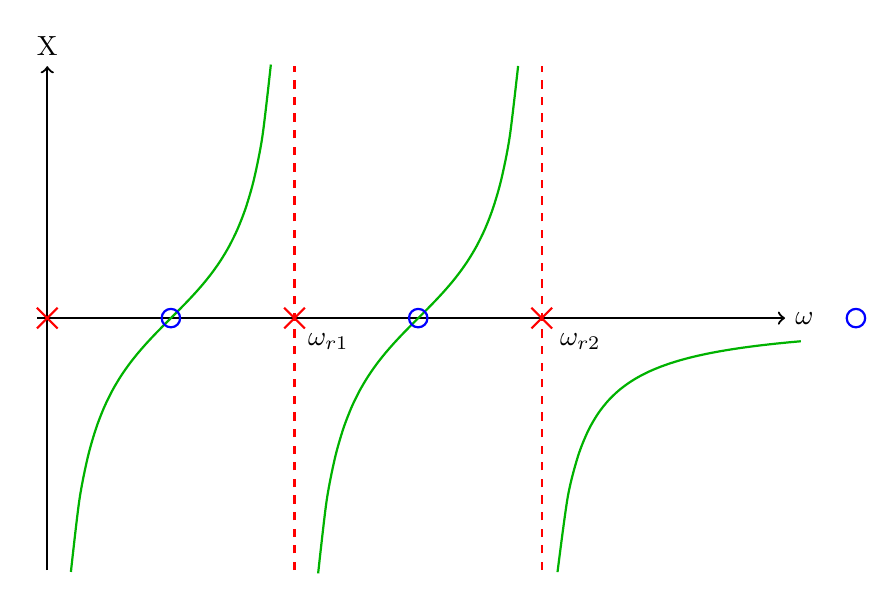
\begin{tikzpicture}[domain=0:4, smooth]
% Achsen
\draw[->, thick] (-1.7,0) -- +(9.5,0) node[right] {$\omega$}; % Horizontal
\draw[->, thick] (-1.57,-3.2) -- +(0,6.4) node[above] {X}; % Vertikal

% Plots
\draw[color=green!70!black, thick] plot[domain=-1.27:1.27] (\x,{tan(\x r)}) node[right] {}; % Erster Tan
\draw[color=green!70!black, thick] plot[domain=1.87:4.41] (\x,{tan(\x r)}) node[right] {}; % zweiter Tan
\draw[color=green!70!black, thick] plot[domain=4.91:8] (\x,{-1/(\x - 4.6)}) node[right] {}; % letzte kurve

% Poolstellen
\draw[dashed, thick, draw=red] (1.57,-3.2) -- +(0,6.4); % Poolstelle 1
\draw[dashed, thick, draw=red] (4.71,-3.2) -- +(0,6.4); % Poolstelle 2

\node[cross out, draw=red, thick] at (-1.57,0) {};

\node[cross out, draw=red, thick] (wr1) at (1.57,0) {};
\node at(2,-0.3) {$\omega_{r1}$};

\node[cross out, draw=red, thick] at (4.71,0) {};
\node at (5.2,-0.3) {$\omega_{r2}$};

% Nullstellen
\node[rounded rectangle, draw=blue, thick] at(0,0) {};
\node[rounded rectangle, draw=blue, thick] at(3.141,0) {};
\node[rounded rectangle, draw=blue, thick] at(8.7,0) {};


\end{tikzpicture}
